\documentclass[a4paper,12pt]{report}
%general packages
\usepackage[T2A]{fontenc}
\usepackage[utf8]{inputenc}
\usepackage[english,russian]{babel}
\usepackage{circuitikz}
\usepackage{wrapfig}
\usepackage{makecell}
\usepackage{tabularx}
\usepackage{graphicx}
\usepackage{gensymb}
\usepackage{cancel} %cancel symbol
\usepackage{amsmath,amsfonts,amssymb,amsthm,mathtools}

%fancy header + geometry
\usepackage{fancyhdr}
\usepackage[a4paper,includehead,nomarginpar,left=15mm,right=15mm,top=15mm,headheight=10mm,bottom=20mm]{geometry}

%pgfplots
\usepackage{pgfplots}
\usepackage{pgfkeys}
\pgfplotsset{compat=1.12}
\usepackage{mathrsfs}

%multi column text
\usepackage{blindtext}
\usepackage{multicol}

%tikz (draw)
\usepackage{tikz}
\usepackage{pstricks-add}
\usetikzlibrary{intersections}
\usetikzlibrary{arrows.meta}
\usetikzlibrary{calc,angles,positioning}
\usetikzlibrary{arrows}
\usepackage{float}

%parskip settings
\parindent=0ex
\setlength{\parskip}{\baselineskip}%
\setlength{\parindent}{0pt}%

%fancy notation for sets
\newcommand{\R}{{\mathbb R}}
\newcommand{\N}{{\mathbb N}}
\newcommand{\fancy}[1]{{\mathbb{#1}}}
%sgn function
\DeclareMathOperator{\sgn}{sgn}

% intersection and union symbols
\newcommand{\uni}{\cup}
\newcommand{\inter}{\cap}
\newcommand{\re}{\text{Re}}
\newcommand{\const}{\text{const}}

\renewcommand{\footrulewidth}{0.4pt}

%\newcommand{\celsius}{$\ ^\circ C$}

%environments

\newtheorem{problem}{Задача}[]
\newenvironment{sol}{\paragraph{Решение}}{}
\renewcommand\thesection{\arabic{section}}

\usepackage{titlesec}
\titlespacing*{\section}
{0cm}{\baselineskip}{0pt}
\titlespacing*{\subsection}
{0pt}{0.1\baselineskip}{0.1\baselineskip}
\titlespacing*{\paragraph}
{0pt}{0.1\baselineskip}{\baselineskip}

\setcounter{secnumdepth}{0}

\begin{document}
	

\begin{titlepage}
	\begin{center}
		МОСКОВСКИЙ ФИЗИКО-ТЕХНИЧЕСКИЙ ИНСТИТУТ (НАЦИОНАЛЬНЫЙ ИССЛЕДОВАТЕЛЬСКИЙ УНИВЕРСИТЕТ) \\
		
		
		\hfill \break
		Факультет обшей и прикладной физики\\
		\vspace{2.5cm}
		\large{\textbf{Отчёт по лабораторной работе 1.2.5 <<Исследование прецессии уравновешенного гороскопа>>}}\\
		\hfill \break
		\\
	\end{center}
	
	\begin{flushright}
		Выполнил:\\
		Студент гр. Б02-304\\
		Головинов. Г.А.
	\end{flushright}
	
	\vspace{7cm}
	
	\begin{center}
		
\includegraphics[width=0.15\linewidth]{uni}
	\end{center}
	

	

	\vfill
	
	\begin{center} Долгопрудный, 2023 \end{center}
	
	\thispagestyle{empty}
	
\end{titlepage}


	\newpage
	%\pagenumbering{arabic}
    \pagestyle{fancy}

    \fancyhead{}
    \fancyfoot{}
    \fancyhead[L]{\rightmark}
    \fancyhead[R]{\thepage}
    \fancyfoot[R]{Работа 2.2.5 --- Определение вязкости жидкости}

    \section*{Аннотация}
        \paragraph*{Цель работы:} 1) определить вязкость дистиллированной воды по измерению объема жидкости, протекшей через капилляр; 2) определение вязкости других жидкостей путём сравнения скорости их протекания со скоростью протекания воды.
        \paragraph*{В работе используются:} сосуд Мариотта; капиллярная трубка; мензурка; секундомер; микроскоп.
    \vspace{0.5cm}
    \hrule
    \begin{multicols}{2}
        \section{Основные теоретические сведения}
        Воспользуемся формулой Пуазейля:
        \begin{equation}
            \label{Poiseuille}
            Q=\frac{\Delta p}{\Delta l}\cdot \frac{\pi R^4}{8\eta}
        \end{equation}
        где $Q$ --- расход жидкости $[\text{m}^3/\text{s}]$, $R$ --- радиус трубки, $\Delta p$ --- разница давлений на концах рассматриваемого участка длиной $\Delta l$, $\eta$ --- вязкость жидкости.

        При малых скоростях течение в трубке ламинарное. При больших скоростях слои начинают перемешиваться, такое течение называется турбулентным. Характер течения зависит от соотношения между кинетической энергией среды и работой сил вязкости. Если первая величина сильно меньше второй, то течение остается ламинарным (энергия как бы подавляет вязкость). Отношение этих величин для некоторого объема среды определяет безразмерное число Рейнольдса:
        \begin{equation}
            \label{raynolds}
            \re=\frac{v R \rho}{\eta}
        \end{equation}
        где $v$ --- характерная скорость течения, $R$ --- радиус трубки (или любой другой характерный размер), $\rho$ --- плотность среды, $\eta$ --- вязкость. 

        В гладких трубках круглого сечения переход от ламинарного к турбулентному течению происходит при $\re\approx 1000$. Число Рейнольдса нужно именно для этого: перед применением формулы Пуазейля \eqref{Poiseuille} стоит убедиться, что течение ламинарное.

        Ламинарное течение при переходе из сосуда в капилляр устанавливается не сразу, а после того, как жидкость пройдет расстояние
        \begin{equation}
            \label{a}
            a\approx 0.2 R \cdot \re
        \end{equation}
        Если длина капилляра много раз расстояния $a$, то можно считать течение в нем ламинарным.
    \end{multicols}
    \hrule
    \begin{multicols}{2}
        \subsection*{Измерение вязкости дистиллированной воды.}
        Для измерения вязкости воды используется сосуд Мариотта, схема установки приведена на рисунке \ref{fig:ustanovka1}
        
        Особенность сосуда Мариотта заключается в том, что разница давления на концах капилляра зависит только от высоты $h$ между низом трубки B и осью капилляра. Кроме того, необходимо учесть, что поверхностное натяжение несколько уменьшает разницу давления.
        \begin{figure}[H]
            \centering
            \label{fig:ustanovka1}
            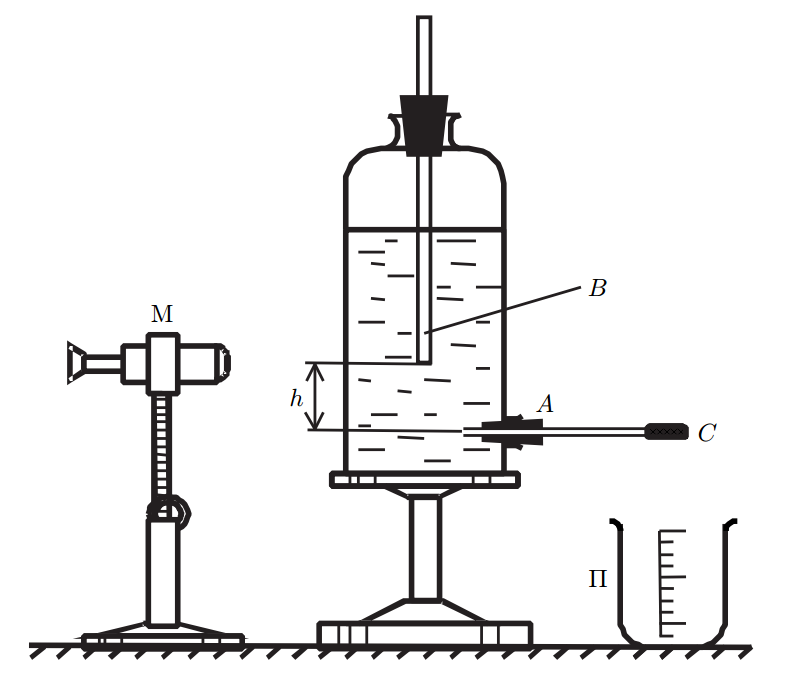
\includegraphics[width=0.75\columnwidth]{../img/ustanovka1.png}
            \caption{Схема установки с сосудом Мариотта.}
        \end{figure}
    \end{multicols}
    \newpage
    \begin{multicols}{2}
        \subsection*{Измерение вязкости водного раствора глицерина вискозиметром.}
        Получив из предыдущего пункта вязкость воды, относительно нее можно получить вязкость других жидкостей. В случае нашей работы это 10-,20-,30-\% раствор глицерина. Для этого нам понадобится измерить время, за которое каждая жидкость вытекает из вискозиметра (а точнее верхняя граница проходит через определенные границы).

        Разность давления в вискозиметре выражается как $\Delta p = \rho g h(V)$, где $h(V)$ --- функция высоты столба от объема, она одинаковая дла каждой жидкости и определяется формой сосуда. Тогда (учитывая что течение ламинарное) можно воспользоваться формулой Пуазейля:
        \begin{equation*}
            -\frac{dV}{dt}=\frac{\rho g h(V)}{l}\cdot\frac{\pi R^4}{\eta}
        \end{equation*}
        тогда можно разделить переменные:
        \begin{equation*}
            -\frac{8 l}{\pi R^4}\cdot \frac{dV}{h(V)}=\frac{\rho g}{\eta}dt
        \end{equation*}
        Пусть первой границе соответствует объем $V_1$, а второй --- $V_2$. Время пусть меняется от $t=0$ до некоторого $t_0$. Тогда проинтегрировав получим:
        \begin{gather}
            \frac{8l}{\pi R^4}\int_{V_1}^{V_2}\frac{dV}{h(V)}=-\int_{0}^{t_0}\frac{\rho g}{\eta}dt \nonumber \\
            \frac{\rho}{\eta}t = \const \label{connst}
        \end{gather}
        константа в левой части целиком определяется сосудом и не зависит от жидкости. Получается, меняя жидкость, величина в правой части сохраняется. Зная времена для каждой жидкости и их плотности можно получить ее вязкость. Конечное выражение для некоторой жидкости $x$ через воду (индекс 0):
        \begin{equation}
            \label{final eta}
            \eta_x=\eta_0\cdot\frac{\rho_x}{\rho_0}\cdot\frac{t_x}{t_0}
        \end{equation}
    \end{multicols}
    \vspace{2mm}
    \hrule
    \begin{multicols}{2}
        \section{Обработка результатов}
        Для нахождения вязкости воды были взяты измерения для 6 различных высот $h$. Полученные данные приведены в виде таблиц в приложении.

        Для определения $\Delta h$ мы медленно уменьшали $h$ до того момента, как вода не перестанет капать из капилляра. Это произошло на высоте порядка 10-12 mm. Будем считать $\Delta h = 11\pm 1$ мм.
        %4.8489003798298553963432654241014e-4

        В результате имеем довольно плохие точки: явно видно, что пересечение линейной части графика с осью ординат больше нуля, что значит, что жидкость вытекала бы даже без избыточного давления. Однако экспериментально видно, что при высоте $h\approx 11 \ \text{мм}$ жидкость течь перестает

        Это приводит к тому, что полученная вязкость воды совсем не соответствует табличным значениям. Скорее всего, виной этому либо проблема с установкой, либо кривые руки автора.

        Далее для определения вязкости растворов возьмем в качестве вязкости воды табличное значение с погрешностью в 5\%:

        \begin{gather*}
            \eta = (0.94 \pm 0.05) \cdot 10^{-3} \ \text{Па}\cdot \text{с}
        \end{gather*}

        Тогда с помощью вискозиметра по полученному времени протекания получим вязкости для растворов глицерина:

        \begin{gather*}
            \eta_1 = (1.33 \pm 0.09) \cdot 10^{-3} \ \text{Па}\cdot \text{с} \\
            \eta_2 = (1.96 \pm 0.11) \cdot 10^{-3} \ \text{Па}\cdot \text{с} \\ 
            \eta_3 = (2.47 \pm 0.13) \cdot 10^{-3} \ \text{Па}\cdot \text{с}
        \end{gather*}

    \end{multicols}

    \newpage

    \section{Выводы}

    \begin{multicols}{2}
        В результате работы вязкость дистиллированной воды получена не была ввиду неисправности установки или кривых рук автора. Однако используя табличное значения для вязкости дистиллированной воды с помощью вискозиметра удалось определить вязкость раствора глицерина с достаточно большой точностью. Лишь 20\% раствор вышел за пределы $\pm 1 \sigma$.
    \end{multicols}

    \hrule

    \section{Приложение}

    \begin{figure}[H]
        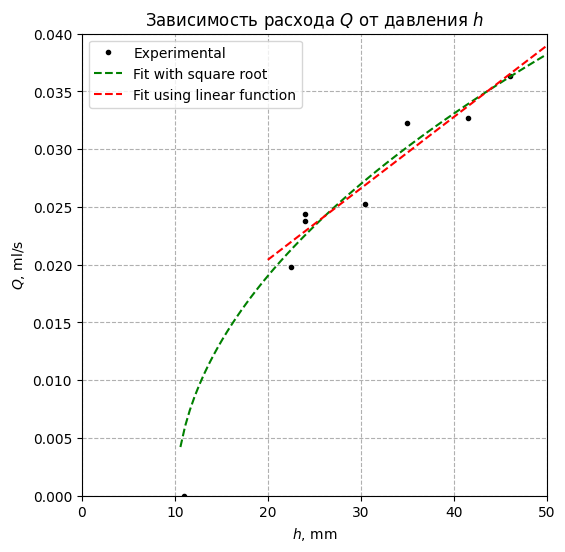
\includegraphics[width=0.75\columnwidth]{../img/output.png}
        \centering
        \label{fig:experimental}
        \caption{Аппроксимация и полученные экспериментальные точки.}
    \end{figure}

    \newpage

    %\begin{multicols}{2}

        \begin{table}[H]
            \centering
            \begin{tabular}{|c|c|c|c|c|}
                \hline
                $N$ опыта & $t$, с & $V$, мл & $Q$, мл/c & $\Delta h$, мм \\
                \hline
                1 & 610 & 20 & 0.0328 & 41.5 \\
                \hline
                2 & 550 & 20 & 0.0364 & 46 \\
                \hline
                3 & 410 & 10 & 0.0244 & 24 \\
                \hline
                4 & 630 & 15 & 0.0238 & 24 \\
                \hline
                5 & 505 & 10 & 0.0198 & 22.5 \\
                \hline
                6 & 792 & 20 & 0.0253 & 30.5 \\
                \hline
                7 & 310 & 10 & 0.0323 & 35 \\
                \hline
            \end{tabular}
            \caption{Результаты измерений потока жидкости через капилляр.}
        \end{table}

        \begin{table}[H]
            \centering
            \begin{tabular}{|c|c|c|c|c|}
                \hline
                Содержание & 0\% & 10\% & 20\% & 30\% \\
                \hline
                $t_1$ & 8.69 & 11.68 & 17.03 & 20.97 \\
                \hline
                $t_2$ & 8.80 & 11.80 & 17.01 & 21.16 \\
                \hline
                $t_3$ & 8.39 & 11.68 & 17.14 & 21.25 \\
                \hline
                $t_4$ & 8.62 & 11.64 & 17.50 & 20.97 \\
                \hline
                $t_5$ & 8.61 & 12.75 & 17.12 & 20.99 \\
                \hline
            \end{tabular}
            \caption{Результаты измерений времени вытекания жидкости через вискозиметр.}
        \end{table}
    %\end{multicols}
\end{document}
